\section{Sesión 13}

\begin{teorema} (Criterio de Kummer)
	Sea $\sum a_n$ una serie de términos positivos. Sea $\sum b_n$ una serie divergente $\ni b_n>0$. Además, considere: 
	$$\alpha =\lim_{n\to\infty}\left(\frac{1}{b_n}\cdot \frac{a_n}{a_{n+1}}-\frac{1}{b_{n+1}}\right)$$
	\begin{enumerate}
		\item Si $\alpha >0\implies \sum a_n$ converge. 
		\item Si $\alpha <0\implies \sum a_n$ diverge. 
		\item Si $\alpha =0$, el criterio no es concluyente. 
	\end{enumerate}
\end{teorema}

\begin{teorema}(Criterio de comparación en el límite)
	Si $\sum a_n$ y $\sum b_n$ sobre series de términos positivos y si $0<\lim_{n\to\infty}a_n/b_n<\infty\implies$ ambas series convergen o divergen. 
\end{teorema}

\begin{teorema}(Leibniz- Series alternantes)
	Supionga que $(a_n)$ es una sucesión decreciente de números positivos $\ni \lim_{n\to\infty}a_n=0$. Entonces, $\sum_{n=1}^{\infty} (-1)^{n+1} a_n$ converge. 
\end{teorema}


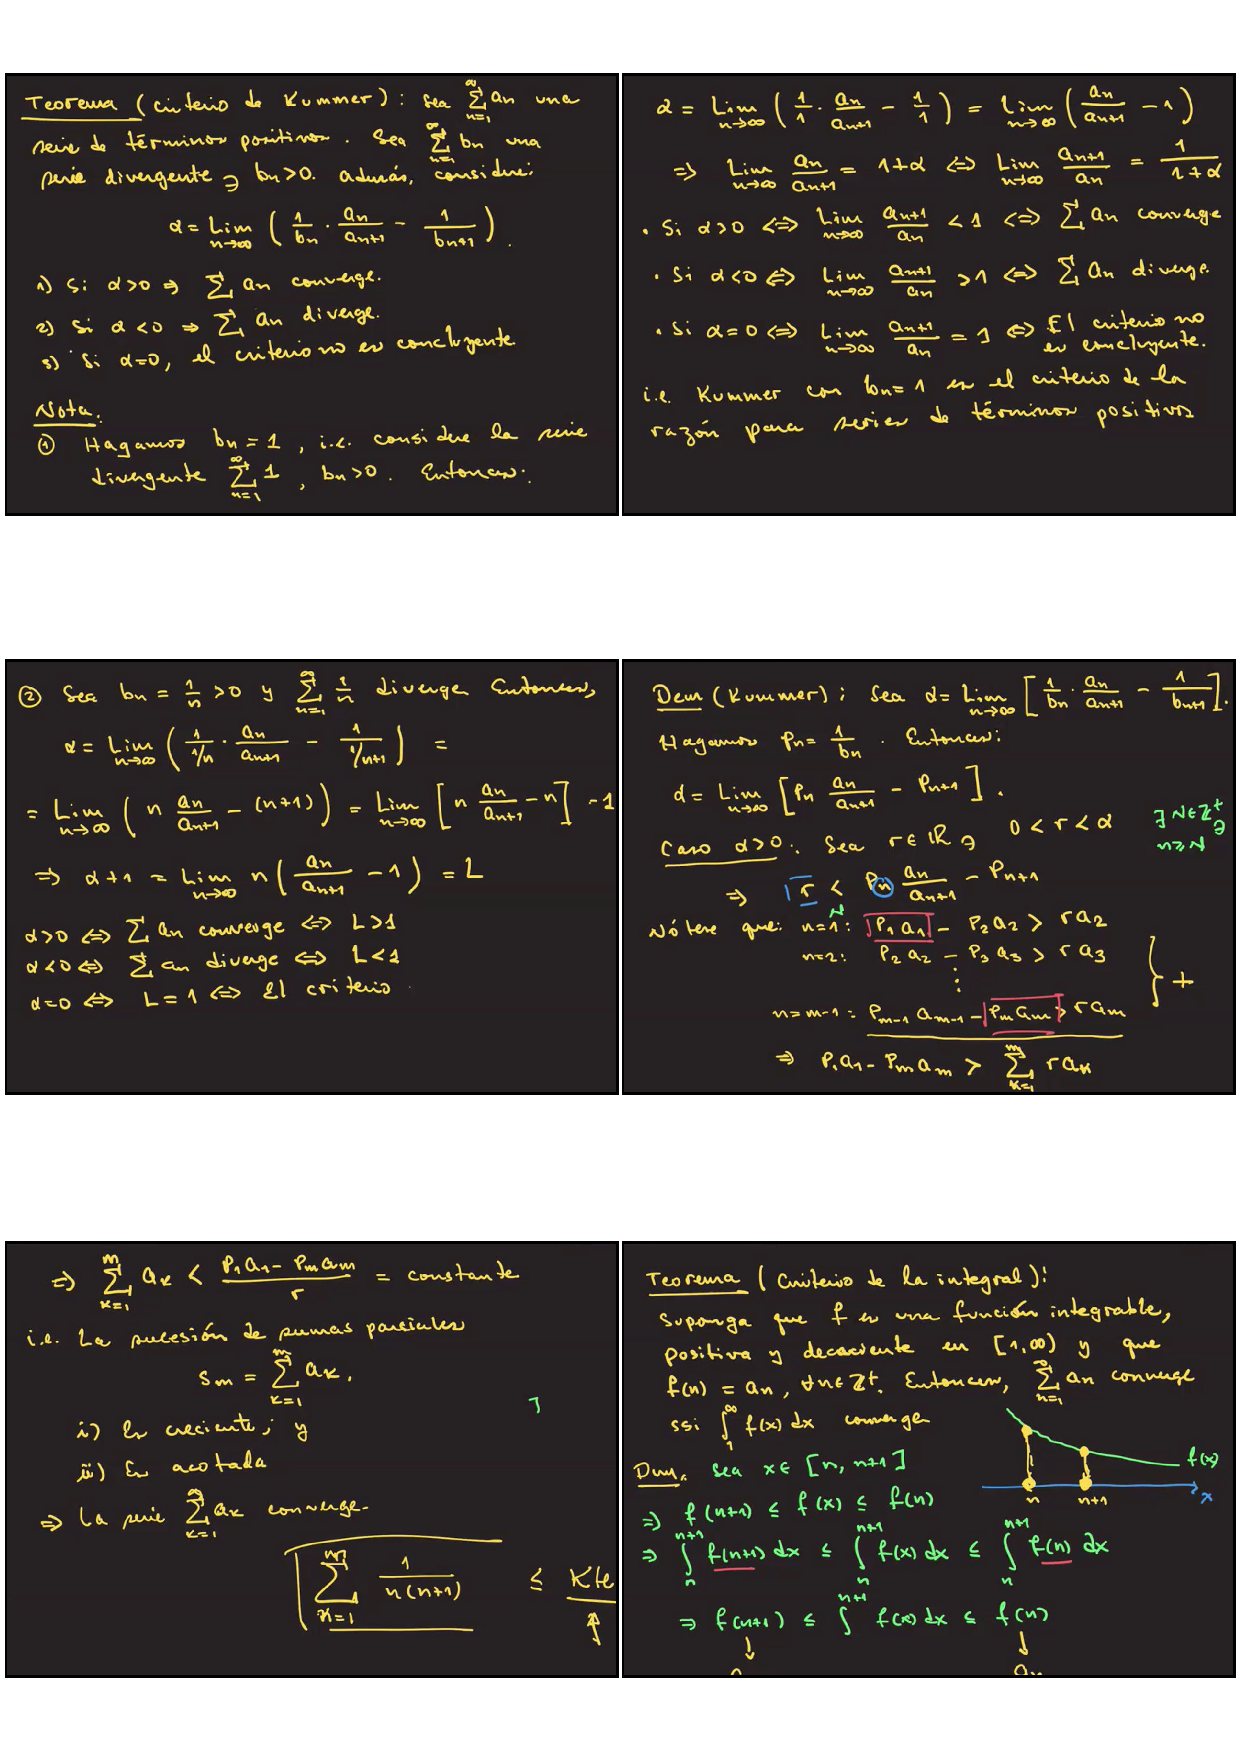
\includepdf[pages=-]{apendices/s13.pdf}